\documentclass[12pt]{article}
\usepackage{palatino}
\usepackage{fullpage}
\usepackage{graphicx}
\usepackage{enumitem}
\usepackage{multirow}
\usepackage{latexsym}
\usepackage{tikz,pgfplots} 
\usepackage{booktabs}
\usetikzlibrary{arrows,automata}

\usepackage{color}
\usepackage{amsmath,amssymb}
\usepackage[utf8]{inputenc}
\pagestyle{empty}

\setlength{\parindent}{0in}
\setlength{\parskip}{.1in}

\newcounter{showsolution}
\setcounter{showsolution}{1}
\newcommand{\solution}[2]{\ifnum\value{showsolution}>0{\textcolor{blue}{#1}}\else{#2}\fi}

\newcounter{QuestionCounter}
%\newcommand{\Question}[1]{\refstepcounter{QuestionCounter} {\bf Question \arabic{QuestionCounter}}. [#1 points] }

\newcommand{\Question}[2]{\refstepcounter{QuestionCounter} \textbf{\Large {Q\arabic{QuestionCounter}}. #1\hfill\textit{#2 points}}}

\begin{document}

{\ }
\vskip 1in

\centerline{\Huge\bf First Midterm Exam}
\vskip .5in
\centerline{\LARGE\bf 601.467/667 Introduction to Human Language Technology}
\vskip .2in
\centerline{\Large Fall 2024}
\vskip .1in
\centerline{\Large Johns Hopkins University}
\vskip .1in
\centerline{\Large Co-ordinator: Philipp Koehn}
\vskip .3in
\centerline{\Large 3 October 2024}
\vskip 1in
\centerline{\Large Complete all questions.}
\vskip .2in
\centerline{\Large Use additional paper if needed.}
\vskip .2in
\centerline{\Large Time: 75 minutes.}
\vskip 1in
\centerline{\Large Name of student: {\rule{3in}{0.4pt}}}

%\newpage
%\Question{\Large Language Modeling}{10}

%\begin{enumerate}
%\item Why did the chicken cross the road?\hfill{\em (30 points)}
%\solution{to get to the other side}{\vspace{7cm}}
%\end{enumerate}

%\newpage 

%\Question{\Large Morphology}{10}

%\begin{enumerate}
%\item Why did the chicken cross the road?\hfill{\em (10 points)}
%\solution{to get to the other side}{\vspace{7cm}}
%\end{enumerate}

%%%%%%%%%%%%%%%%%%%%%%%%%%%%%%%%%%%%%%%%%%%%%%%%%%
\newpage
\Question{\Large Syntax}{20}

\paragraph{Formal Language Theory}
\begin{itemize}

\item[1.] We defined a formal language as $\cal{L}$ as a set of words over an alphabet $\Sigma$, where the words are drawn from $\Sigma^*$.
\begin{itemize}
    \item[a.] What is meant by $\Sigma^*$?\hfill{\em (1 point)}\\\\

    \item[b.] Give an example of a $\Sigma$ and a language drawn from that set, such that $\cal{L}$ is a strict subset of $\Sigma$.\hfill{\em (1 point)}\\\\
    \item[c.] Suppose we define
    \begin{eqnarray*}
    \Sigma_1 &=&\{0, 1, 2, 3, 4, 5, 6, 7, 8, 9\} \\
    \Sigma_2 &=&\Sigma_1 \cup \{-\} \\
    \Sigma_3 &=&\Sigma_2 \cup \{.\}
    \end{eqnarray*}
    What are three languages that could sensibly be defined over these alphabets?\\\\
    ${\cal{L}}_1$ = \\\\ 
    ${\cal{L}}_2$ = \\\\
    ${\cal{L}}_3$ = \hfill{\em (3 points)}\\\\
    \item[d.] For each language you have defined (${\cal{L_1, L_2, L_3}}$), give an example of a string that is \emph{in} that language and a string that is \emph{out} of the language. Recall that each string must be valid according to its respective alphabet.\hfill{\em (6 points)}\\\\
\end{itemize}

\solution{A language is a set of strings over a finite alphabet, $\Sigma$. 
It is a subset of the complete set of strings, $\Sigma^*$.
Examples include the set of valid URLs, the set of floating point numbers, and the set of English-German code-switched sentences.
A string $s$ is not in a language if $s\in\Sigma^*$ and $s\notin{\cal{L}}.$ \vspace{2cm}}
{\vspace{55mm}}



\item[2.]
The Chomsky hierarchy defines four language classes of increasing power, corresponding to four contraints on the rule format. 
Draw a line between connecting each rule format in the Chomsky hierarchy with the associated language class.
A, B, and C are nonterminal symbols, while $\alpha$, $\beta$, and $\gamma$ represent a mix of any number of nonterminal and terminal symbols (with a length of at least one). \textbf{Note}: one entry in each column is a fake.
\hfill{\em (4 points, 1 for each correct link)}\linebreak

\begin{table}[h]
\centering
\begin{tabular}{|l|p{2in}|p{2in}|}
\toprule
\textbf{power} & \textbf{rule format} & \textbf{language class} \\
\midrule
& & \\
& A\ $\rightarrow$b\ C
& context-sensitive
\\ & & \\
& A\ $\rightarrow\alpha$
& context-laden
\\ & & \\
& $\alpha$A$\beta\rightarrow\alpha\gamma\beta$
& recursively enumerable
\\ & & \\
& $\alpha\rightarrow\beta$
& regular
\\ & & \\
& $\alpha$A$\beta\rightarrow \gamma$
& context-free
\\ & & \\
\bottomrule
\end{tabular}
\end{table}

\solution{$\alpha\rightarrow\beta$ and ``context-laden'' are fake. The rules are in order from regular, to context free, to context sensitive, to recursively enumerable.}

\item[3.] Number the above language classes in terms of their descriptive power, with (1) being the most powerful, and (4) being the least powerful.\hfill{\em (2 points)}\linebreak

\solution{(1) recursively enumerable (2) context-sensitive (3) context-free (4) regular \vspace{2cm}}{\vspace{2cm}}




\item[4.] Explain the concept of ``natural language''. Given your definition, what are unnatural languages? Give an example of one. What is the use of formal language theory with respect to both types?\hfill{\em (3 points)}\linebreak

\solution{Natural languages are human languages, in contrast to synthetic or engineered languages or specifications like Python or HTML. 
They can both be split into groups of ``valid'' and ``invalid'' sentences, though the split is fuzzier in natural languages. 
Formal language theory can be used to describe the structure of both types of languages, though its application to natural languages is not perfect.\vspace{3cm}}{\vspace{3cm}}



\item[5.] What is the first sentence of the Penn Treebank?\hfill{\em (1 point extra credit)}\linebreak
\solution{\emph{Pierre Vinken, 61 years old, will join the board as a nonexecutive director Nov.\ 29.}. Full credit given if the sentence is more-or-less correct; one point of credit is given if the major gist is there.}{}


\end{itemize}

%%%%%%%%%%%%%%%%%%%%%%%%%%%%%%%%%%%%%%%%%%%%%%%%%%
\newpage
\Question{\Large Semantics}{15}

\begin{enumerate}
\item Give an example of a word that is \emph{polysemous} and a word that is \emph{homonymous}, and explain why this is the case. \hfill{\em (10 points)}
\solution{The word "fluke" can be used for both polysemy and homonymy.  For the former, it may refer to "an unusual event" or "a type of flat fish", from unrelated roots from different languages (homonymy). For the latter, the meaning of "a flat-shaped anchor" was coined due to the similarity with the fish (therefore, polysemy). }{\vspace{7cm}}

\item Consider the sentences "I baked the cake with the oven" and "The oven baked the cake": characterize what syntactic and semantic roles the word "oven" has in each with respect to the verb "baked". \hfill{\em (5 points)}
\solution{In the first sentence, "oven" is part of a prepositional phrase (i.e. the dependent of "with") attached to the verb, while in the second sentence it is the verb's direct object. In both cases, its semantic role is "instrument", something non-intentionally performing an action.}{\vspace{7cm}}
\end{enumerate}

%\newpage
%\Question{\Large Deep Learning}{20}

%\begin{enumerate}
%\item Why did the chicken cross the road?\hfill{\em (20 points)}
%\solution{to get to the other side}{\vspace{7cm}}
%\end{enumerate}

\newpage
\Question{\Large Information Retrieval}{10}

\begin{enumerate}
\item What is the difference between queries and topics?\hfill{\em (2 points)}
\solution{
A topic conveys the exact information that a user is looking for; a query is a realization of a search topic, which may be short, ambiguous, or even not present to the search engine (e.g., in a recommendation system where a user profile is an implicit query). 
}{\vspace{3cm}}

\item What information does relevance judgment capture in the Cranfield paradigm? {\em (3~points)}
\solution{
Relevance judgments record the accessor/annotator's opinion on whether a document is relevant to the topic. Such judgments are not factual but opinions since a document can be considered relevant for an accessor but not for others. 
}{\vspace{3cm}}

\item Assuming you are designing a search engine for lay people (i.e., people without serious medical training) to search for medical literature with fast query response time, what kind of retrieval model architecture would you like to use and why?  \hfill{\em (5~points)}
\solution{
Option 1 (a better one): learned-sparse retrieval model. Since the search engine needs to respond to queries quickly, learned-sparse retrieval models leverage the inverted index to provide short query latency while using a trained, neural sparse encoder to encode the queries and the documents. Such encoders provide semantic matching capabilities, which can bring the lay-person terms closer to the medical terms (or vice versa). \\
Option 2: statistical retrieval model with dictionaries to match the terminologies between lay-person and medical literature. Statistical models leverage inverted index data structure for fast query latency. However, such models can only match the queries and documents based on their surface form. The system would need to expand or modify the queries or documents to ensure terms on either side are added to the queries or documents to ensure surface form matching is capable of retrieving relevant documents. 
}{\vspace{7cm}}

\end{enumerate}

\newpage
\Question{\Large Distributional Semantics}{15}

\begin{enumerate}
\item From what you know about embedding spaces for words that are learned with methods like CBOW, where would the following words be placed in relation to each other: {\em cat, lion, dog, friendly, dangerous}? \hfill{\em (10 points)}

Put these words into the following box to reflect the distances of word vectors:

\solution{cat, lion, dog next to each other, with cat and dog closest; friendly and dangerous in a different cluster, friendly a bit closer to cat/dog, dangerous a bit closer to lion}{\fbox{%
  \parbox{15.2cm}{%
    \begin{center}
      \vspace{5cm}
    \end{center}
  }%
}}

\vspace{1cm}
\item What is the difference between word embeddings (as learned by CBOW) and word representations in deeper layers of transformer models? Explain this for the example of the word {\em bat} in the following two sentences:\hfill{\em (5~points)}

\begin{itemize}
\item {\em The player hit the ball with the bat out of the ballpark.}
\item {\em The explorer entered the cave where a bat flew just past his head.}
\end{itemize}

\solution{In CBOW word embeddings, the word {\em bat} would have the same fixed vector in both sentences, in deeper transformer layers they would be different, one closer to the representation of {\em racket}, one closer to the representation of {\em bird}.}{}


\end{enumerate}

\newpage
\Question{\Large Information Extraction}{20}

\begin{enumerate}
\item Viterbi Algorithm \hfill{\em (10 points)}

Consider the following fragment of the search graph of the Viterbi algorithm.

\begin{tabular}{p{5cm}p{3.5cm}p{4cm}}
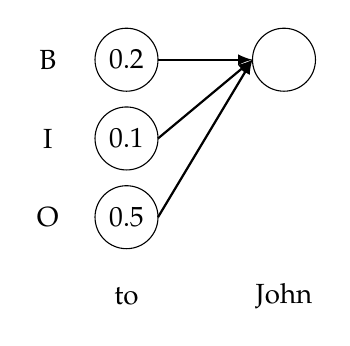
\begin{tikzpicture}
  % Row of circles
  \draw (1,4) circle (0.4) node {0.2};
  \draw (1,3) circle (0.4) node {0.1};
  \draw (1,2) circle (0.4) node {0.5};
  \draw (3,4) circle (0.4);
  % Arrows
  \draw[->,>=latex,thick] (1.4,4) -- (2.6,4);
  \draw[->,>=latex,thick] (1.4,3) -- (2.6,4);
  \draw[->,>=latex,thick] (1.4,2) -- (2.6,4);
  % Labels
  \node at (0,4) {B};
  \node at (0,3) {I};
  \node at (0,2) {O};
  \node at (1,1) {to};
  \node at (3,1) {John};
\end{tikzpicture}
&
\vspace{-3cm}
\begin{tabular}{l}
$p(B|B)$ = 0.1\\
$p(B|I)$ = 0.2\\
$p(B|O)$ = 0.3\\
\end{tabular}
&
\vspace{-3cm}
\begin{tabular}{c}
$p(\text{John}|B)$ = 0.1\\
\end{tabular}
\end{tabular}

Using the Viterbi algorithm and the probabilities from the tables above, how what score and backpointer would the state on the right (corresponding to {\em (I; Smith)} assigned to? Show all your computations that allow you to make that determination.

\solution{
From B: $0.2 \times 0.1 \times 0.1 = 0.002$.\\
From I: $0.1 \times 0.2 \times 0.1 = 0.002$.\\
From O: $0.5 \times 0,3 \times 0.1 = 0.015$.\\
Best is from O, with score 0.015.}{\vspace{4cm}}

\item You were hired by a company to build a chatbot that provides information about the company. It should be able to answer questions like the following:\hfill{\em (10 points)}
\begin{itemize}
\item What is Joe Johnson's cell phone number?
\item Can you give me the email address of Jane Smith in Accounting?
\item I would like to know in which department does Taylor Miller works. Do you have that information?
\end{itemize}
Outline the design of such a chatbot.

\solution{expected answer: store information in a database, use a language model to translate the question into an SQL query, execute the query and return the answer.}{\vspace{7cm}}
\end{enumerate}

\newpage
\Question{\Large Machine Translation}{10}

\begin{enumerate}
\item Below is a bitext of 3 sentence pairs in two fictional languages, Alphian and Censian. Please list ALL the word translation equivalences based on code-breaking principles. {\em (5 points)}
\begin{enumerate}
\item Alphian: ``SAN DOO" translates to Censian: ``ce ti"
\item  Alphian: ``DOO MIO DET" translates to Censian: ``ce bu ma"
\item Alphian: ``FAN MIO DOO" translates to Censian ``ho bu ce"
\end{enumerate}
\solution{SAN = ti, DOO = ce, MIO = bu, DET = ma, FAN = ho}{\vspace{4cm}}

\item Here is a schematic of an recurrent NMT decoder at the $i$-th step, where $c_i$ represents the context vector coming from the encoder, $s_i$ represents the recurrent hidden state, $t_i$ represents the word prediction, and $y_i$ represents the selected word. The state is defined by $s_i = f(s_{i-1}, Ey_{i-1}, c_i)$, where $f(\cdot)$ is a non-linear function. Please explain what might happen to the output translation if $s_i$ is alternatively defined with fewer inputs. {\em (5 points)}
\begin{enumerate}
    \item What happens if $s_i = f(Ey_{i-1}, c_i)$?
    \item What happens if $s_i = f(s_{i-1}, c_i)$?
    \item What happens if $s_i = f(s_{i-1}, Ey_{i-1})$?
\end{enumerate}
\includegraphics[scale=0.4]{mt-decoder.png}
\end{enumerate}
\solution{(a) Missing the previous state $s_{i-1}$ will make this not recurrent. There will be no memory keeping track of previous state, though one might be able to depend on $y_{i-1}$ for that. (b) There is no explicit information about the previously translated word, though this info may be captured by $s_{i-1}$ somewhat. (c) The decoder is completely disconnected from the encoder, so it would just hallucinate without conditioning on the source side. Comment: generally any explanation that seems plausible is fine; the goal is to check whether students understand what is the motivation of each connection in the neural net.}{\vspace{4cm}}

\newpage
\section*{Extra Space}
\newpage
\end{document}

